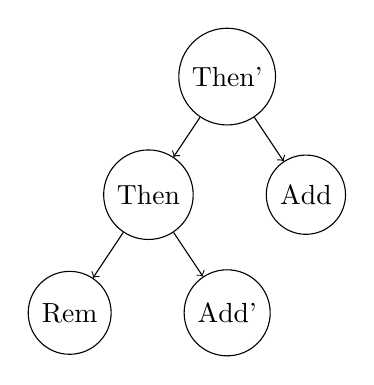
\begin{tikzpicture}
  \node (root) [circle, draw, minimum height=1cm, minimum width=1cm] at (0, 0) {Then'};
  \node (add) [circle, draw, minimum height=1cm, minimum width=1cm] at (1, -1.5) {Add};
  \node (then) [circle, draw, minimum height=1cm, minimum width=1cm] at (-1, -1.5) {Then};
  \node (add-1) [circle, draw, minimum height=1cm, minimum width=1cm] at (0, -3) {Add'};
  \node (rem) [circle, draw, minimum height=1cm, minimum width=1cm] at (-2, -3) {Rem};

  \draw[->] (root) to node[midway, above] {} (add);
  \draw[->] (root) to node[midway, above] {} (then);
  \draw[->] (then) to node[midway, above] {} (add-1);
  \draw[->] (then) to node[midway, above] {} (rem);
\end{tikzpicture}
